\documentclass[12pt]{article}
\usepackage{graphicx}
\usepackage{xcolor}
\usepackage{geometry}
\geometry{margin=1in}

\begin{document}

\begin{center}
\includegraphics[width=0.4\textwidth]{iiitb_logo.png.jpg}
\end{center}

\begin{center}
\textbf{\Large Harshita N Kumar} \\
ID: COMETFWC052
\end{center}

\vspace{0.5cm}

{\color{blue}\section*{Question 11}}

Match the logic gates in Column A with their equivalents in Column B.

\vspace{0.5cm}

\begin{center}
\begin{tabular}{|c|c|}
\hline
\textbf{Column-A} & \textbf{Column-B} \\
\hline
1. AND GATE & P. XOR GATE \\
2. OR GATE  & Q. XNOR GATE \\
3. NOT GATE & R. NAND GATE \\
\hline
\end{tabular}
\end{center}

\vspace{0.3cm}

\begin{center}
\textbf{TABLE 11: Table-1}
\end{center}

\vspace{0.5cm}

a) P-2, Q-4, R-1, S-3 \hspace{1cm}
b) P-4, Q-2, R-1, S-3

\vspace{0.3cm}

c) P-2, Q-4, R-3, S-1 \hspace{1cm}
d) P-4, Q-2, R-3, S-1


\vspace{0.8cm}

{\color{blue}\section*{Question Analysis}}

The AND gate produces output 1 only when both inputs are 1.
The NAND gate is the complement of AND.
Hence, NAND = NOT(AND).

The XOR gate produces output 1 when inputs are different.
The XNOR gate is the complement of XOR.

Using logical relationships:

$Q = (A \cdot B)'$

After comparing the logical behavior of each gate,
the correct matching is:

$P-2,\ Q-4,\ R-3,\ S-1$


\vspace{0.8cm}

{\color{blue}\section*{Truth Table}}

AND Gate: $Q = A \cdot B$

\begin{center}
\begin{tabular}{|c|c|c|}
\hline
A & B & A.B \\
\hline
0 & 0 & 0 \\
0 & 1 & 0 \\
1 & 0 & 0 \\
1 & 1 & 1 \\
\hline
\end{tabular}
\end{center}

NAND Gate: $Q = (A \cdot B)'$

\begin{center}
\begin{tabular}{|c|c|c|}
\hline
A & B & NAND \\
\hline
0 & 0 & 1 \\
0 & 1 & 1 \\
1 & 0 & 1 \\
1 & 1 & 0 \\
\hline
\end{tabular}
\end{center}


\vspace{0.8cm}

{\color{blue}\section*{Hardware Implementation}}

The circuit is implemented using Arduino UNO and IC 7447.
The logical output is displayed on a common anode 7-segment display.

\begin{center}
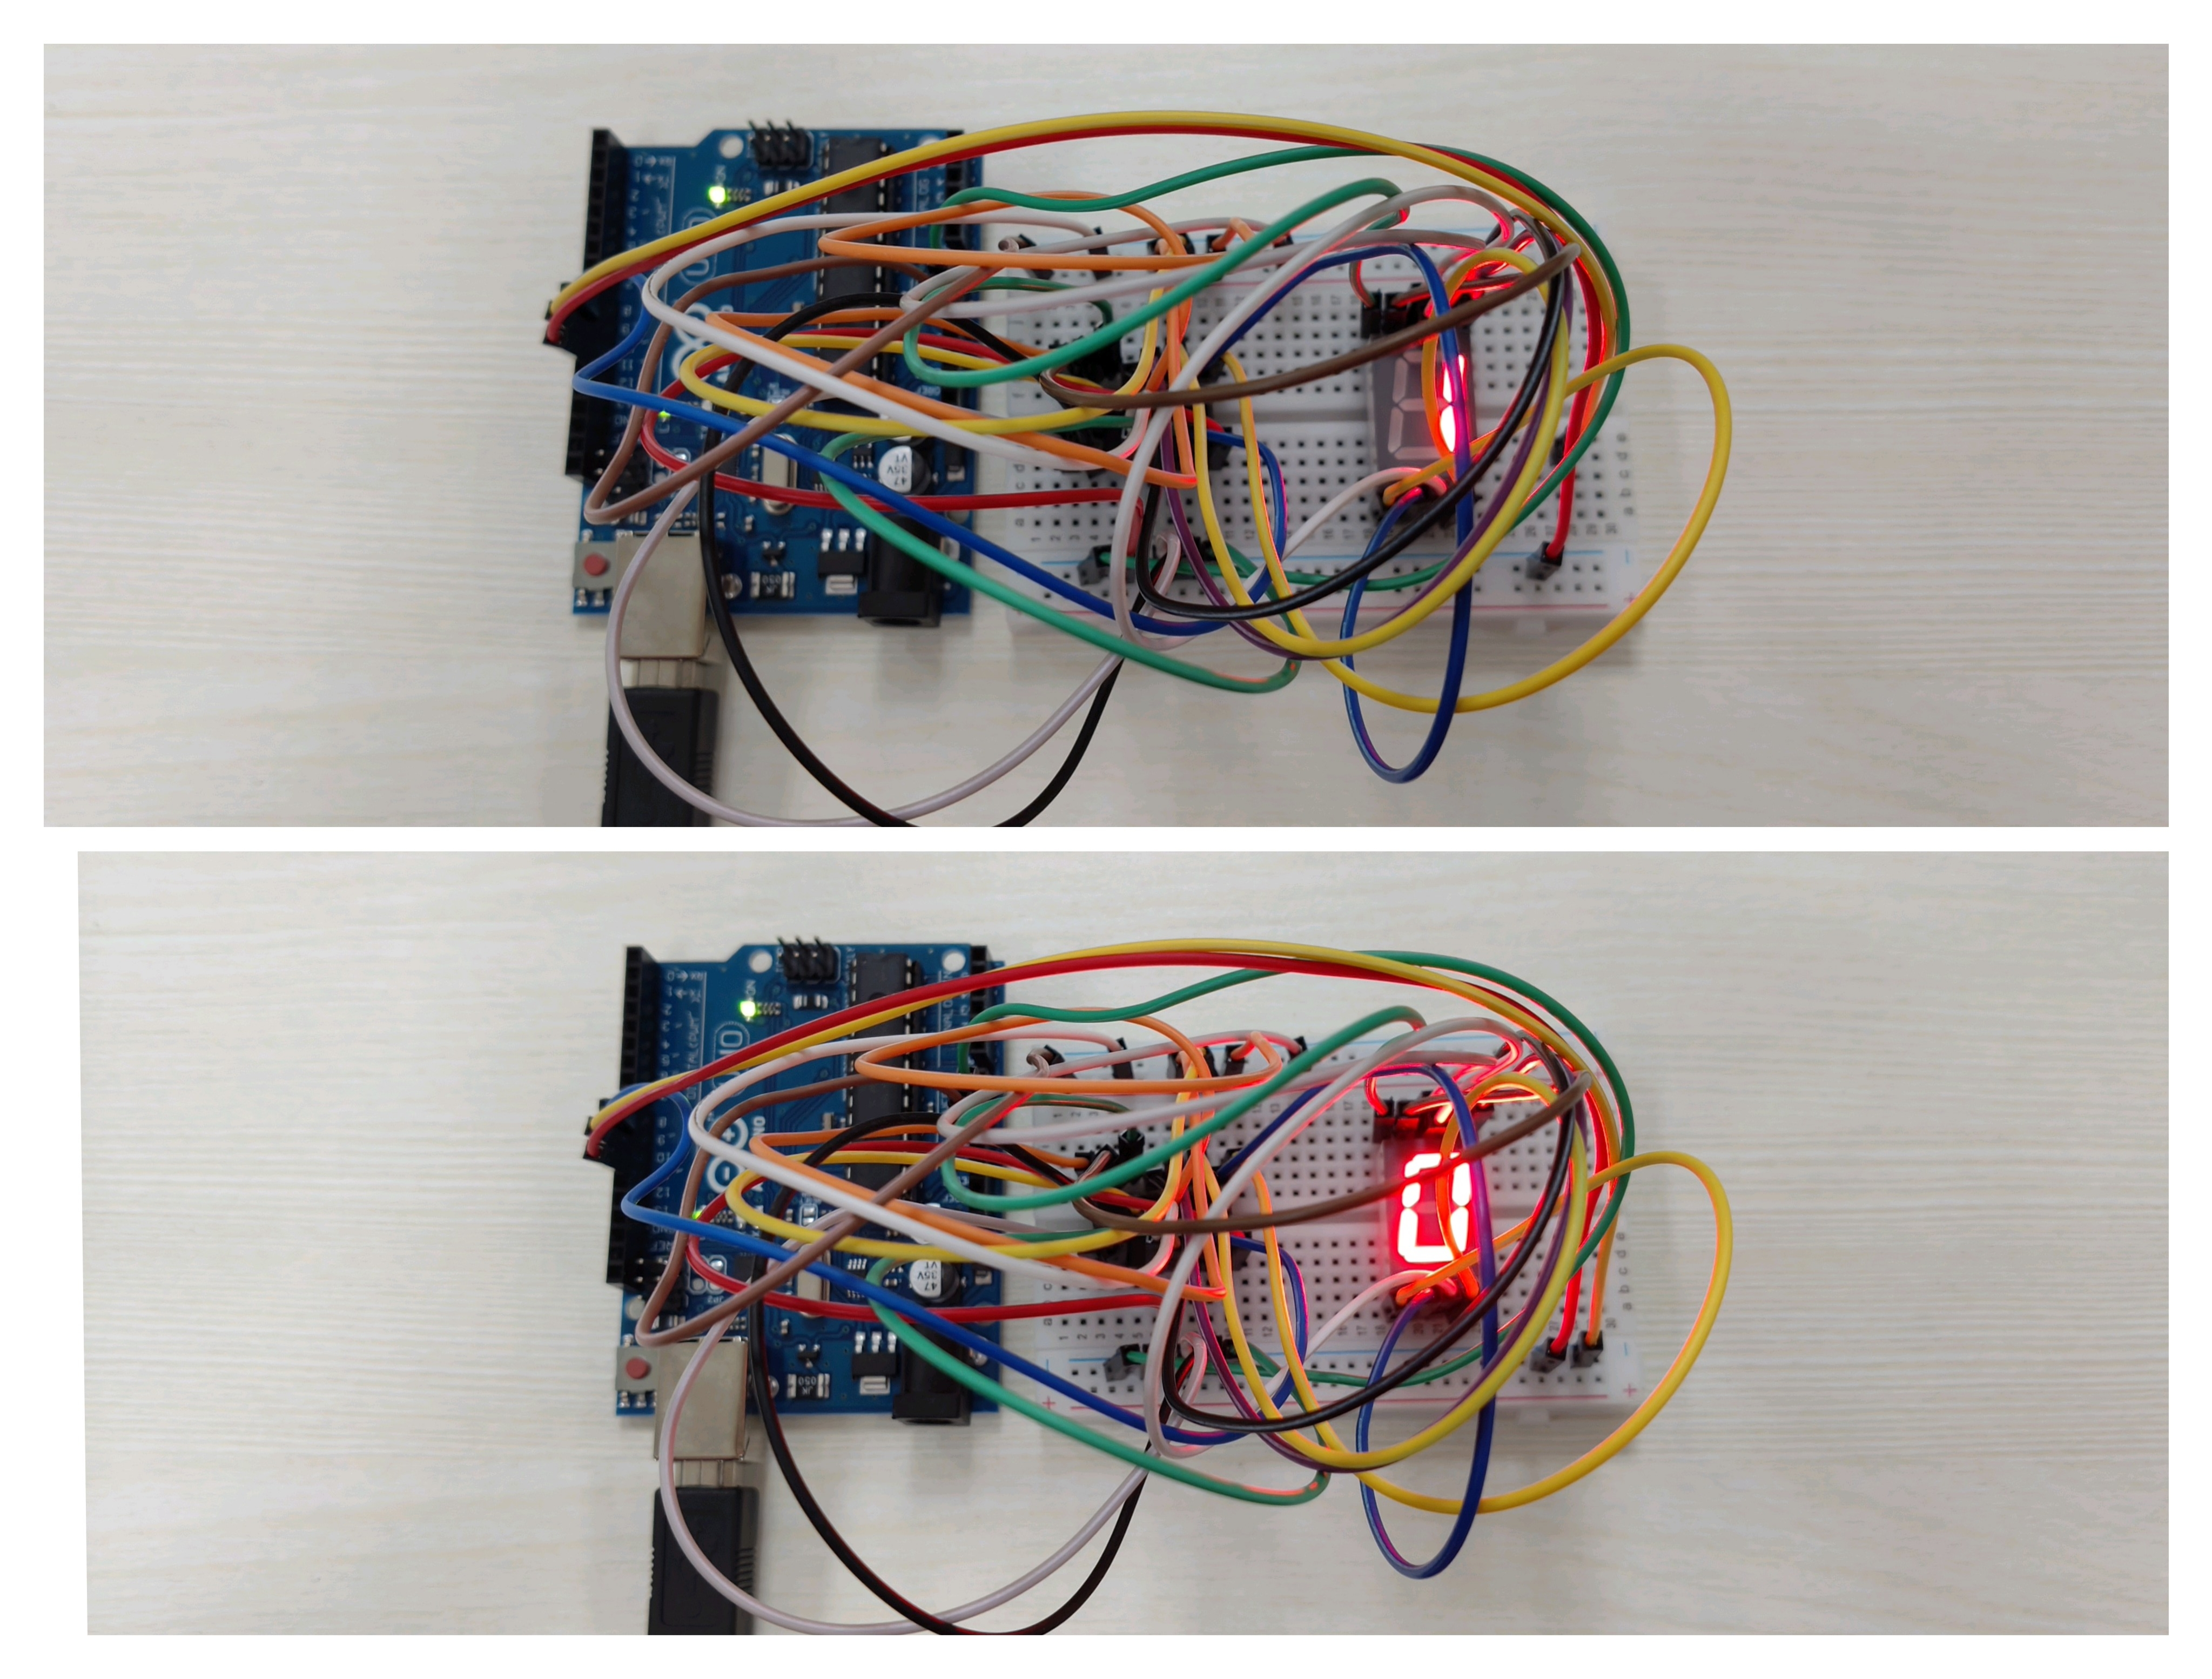
\includegraphics[width=0.8\textwidth]{hardware.jpg}
\end{center}


\vspace{0.8cm}

{\color{blue}\section*{Required Components}}

\begin{itemize}
\item Arduino UNO
\item IC 7447
\item Common Anode 7-Segment
\item Breadboard
\item Jumper wires
\end{itemize}


\vspace{0.8cm}

{\color{blue}\section*{Pin Connections}}

Pin 16 $\rightarrow$ 5V  
Pin 8 $\rightarrow$ GND  
Pin 3,4,5 $\rightarrow$ 5V  

Common Anode $\rightarrow$ 5V  

Segments connected from 7447 output pins through resistors.


\vspace{0.8cm}

{\color{blue}\section*{Logic Description}}

The implemented logic verifies the NAND operation.

Expression: $Q = (A \cdot B)'$

Output is LOW only when both inputs are HIGH.


\vspace{0.8cm}

{\color{blue}\section*{Conclusion}}

The experimental verification confirms the logical equivalence.

Hence the correct answer is verified successfully.

\end{document}
